\documentclass[a4paper]{scrartcl}
\usepackage{mathe-blatt}
\usepackage{graphicx}
\usepackage{listings}
\blattnumeins

\begin{document}

\begin{aufgabe}~

	\begin{enumerate}[a)]
		\item 
			Berechne die Koeffizienten nach der Rekursion
			\begin{align*}
				f[x_i] &:= f_i\\
				f[x_i,\dotsc,x_{i+j}] &:= \f {f[x_{i+1},\dotsc,x_{i+j}]-f[x_i,\dotsc,x_{i+j+1}]}{x_{i+j}-x_i}
			\end{align*}

			\begin{table}[h]
				\centering
				\caption{Dividierte Differenzen: Schema aus der Vorlesung}
				\begin{tabular}{r|rrrrrr}
					-3 & 90 & -73 & 29 & -6 & 1 & 0 \\
					-2 & 17 & -15 & 5 & -1 & 1 & \\
					-1 & 2 & 0 & 1 & 4 & & \\
					 1 & 2 & 3 & 17 & & & \\
					 2 & 5 & 37 & & & & \\
					 3 & 42 & & & & &
				\end{tabular}
			\end{table}
			Es ergibt sich als Newton Darstellung des Polynoms
			\[
				p(x) = 90 - 73(x+3) + 29(x+3)(x+2) - 6(x+3)(x+2)(x+1) + (x+3)(x+2)(x+1)(x-1)
			\]
		\item
			Nutze das Neville-Schema, um die Rekursion
			\begin{align*}
				p_{j,0} &:= f_i \\
				p_{i,j} &:= \f {(x-x_i)p_{i+1,j-1}-(x-x_{i+j})p_{i,j-1}}{x_{i+j}-x_i}
			\end{align*}
			an der Stelle $x=4$ auszuführen.

			\begin{table}[h]
				\centering
				\caption{Neville-Schema zur Auswertung des Interpolationspolynoms}
				\begin{tabular}{r|rrrrrr}
					-3 & 90 & -421 & 797 & -463 & 167 & 167 \\
					-2 & 17 & -73 & 77 & -13 & 167 & \\
					-1 & 2 & 2 & 17 & 137 & & \\
					 1 & 2 & 11 & 113 & & & \\
					 2 & 5 & 79 & & & & \\
					 3 & 42 & & & & &
				\end{tabular}
			\end{table}
			Es ergibt sich also
			\[
				p(4) = 167
			\]
	\end{enumerate}
\end{aufgabe}
\newpage

\begin{aufgabe}
	\begin{enumerate}[a)]
		\item 
			Wir benutzen die Aussage aus b).
			Wir wählen dafür die Stützstellen als $x_0,\dotsc,x_{n-1}$ und $t:=x_n$.
			Es gilt dann
			\[
				f(x_n) - p(x_n) = f[x_0,\dotsc,x_n] \prod_{j=0}^{n-1} (x_n-x_j)
			\]
			Nach dem Satz über punktweise Interpolationsfehler aus der Vorlesung existiert insbesondere ein $\xi\in (a,b)$, so dass gilt
			\[
				p(x_n) - f(x_n) = \f 1{n!} f^{(n)}(\xi) \prod_{j=0}^{n-1} (x_n-x_j)
			\]
			Also gilt für dieses $\xi$:
			\[
				f[x_0,\dotsc,x_n] = \f 1{n!} f^{(n)}(\xi)
			\]
		\item
			Sei $p_{n+1}(x)$ die Interpolierende zu den Stützstellen $x_0,\dotsc,x_{n+1}$ und $p_{n}(x)$ entsprechend die Interpolierende zu den Stützstellen $x_0,\dotsc,x_n$.
			Wegen der hierarchischen Eigenschaft der Newtoninterpolationspolynome gilt:
			\[
				p_{n+1}(x) = p_n(x) + f[x_0,\dotsc,x_{n+1}]\prod_{j=0}^n (x-x_j)
			\]
			Interpoliere nun entsprechend obiger Formel $f(x)$ an den Stützstellen $x_0,\dotsc,x_n,t$.
			Dabei ergibt sich als nächstkleineres Polynom genau $p(x)$.
			Für die Interpolierende gilt dann:
			\[
				\tilde f(x) = p(x) + f[x_0,\dotsc,x_n,t]\prod_{j=0}^n (x-x_j)
			\]
			Da $\tilde f(x) = f(x)$ für $x=t$ folgt sofort die Aussage
			\[
				f(t) - p(t) = f[x_0,\dotsc,x_n,t] \prod_{j=0}^n (t-x_j)
			\]
	\end{enumerate}
\end{aufgabe}

\newpage
	\lstset{basicstyle=\scriptsize}
\setcounter{aufgabe}{3}

\begin{aufgabe}~

	Der Programmcode (Matlab), lautet:
	\begin{lstlisting}[language=matlab]
% Stephan Hilb, 2706616

% Aufgabenteil a)
for n = 4:2:12
    subplot(5,2,n-3);
    
    Xs = -1 + (0:n).*(2/n);
    Ys = 1./(1 + 12*Xs.^2);
    p = polyfit(Xs,Ys,n);
    
    % Ausgabe des Polynoms
    str = '';
    for i = n:-1:1
        str = strcat(str, num2str(p(n-i+1),'%+f'), '*x^', num2str(i));
    end
    str = strcat(str, '+', num2str(p(n+1)))
    
    Xp = linspace(min(Xs),max(Xs),200);
    Yp = polyval(p,Xp);
    
    plot(Xp,Yp,'b-',Xs,Ys,'bo','markersize',4,'markerfacecolor','b');
    
    % Funktion f(x)
    hold on
    Xp = linspace(-1,1,200);
    Yp = 1./(1+12*Xp.^2);
    plot(Xp,Yp,'--r');
    hold off ;
    axis([-1,1,-0.5,1]);
end

% Aufgabenteil b)
for n = 4:2:12
    subplot(5,2,n-2);
    
    Xs = cos((n-(0:n))*pi/n);
    Ys = 1./(1 + 12*Xs.^2);
    p = polyfit(Xs,Ys,n);
    
    % Ausgabe des Polynoms
    str = '';
    for i = n:-1:1
        str = strcat(str, num2str(p(n-i+1),'%+f'), '*x^', num2str(i));
    end
    str = strcat(str, '+', num2str(p(n+1)))
    
    Xp = linspace(min(Xs),max(Xs),200);
    Yp = polyval(p,Xp);
    
    plot(Xp,Yp,'b-',Xs,Ys,'bo','markersize',4,'markerfacecolor','b'); 
    
    % Funktion f(x)
    hold on
    Xp = linspace(-1,1,200);
    Yp = 1./(1+12*Xp.^2);
    plot(Xp,Yp,'--r');   
    hold off;
    axis([-1,1,-0.5,1]);
end
	\end{lstlisting}
		\begin{figure*}[h]
			\centering
			\caption{Interpolationspolynome, links a), rechts b), jeweils für $n\in\{4,6,8,10,12\}$}
			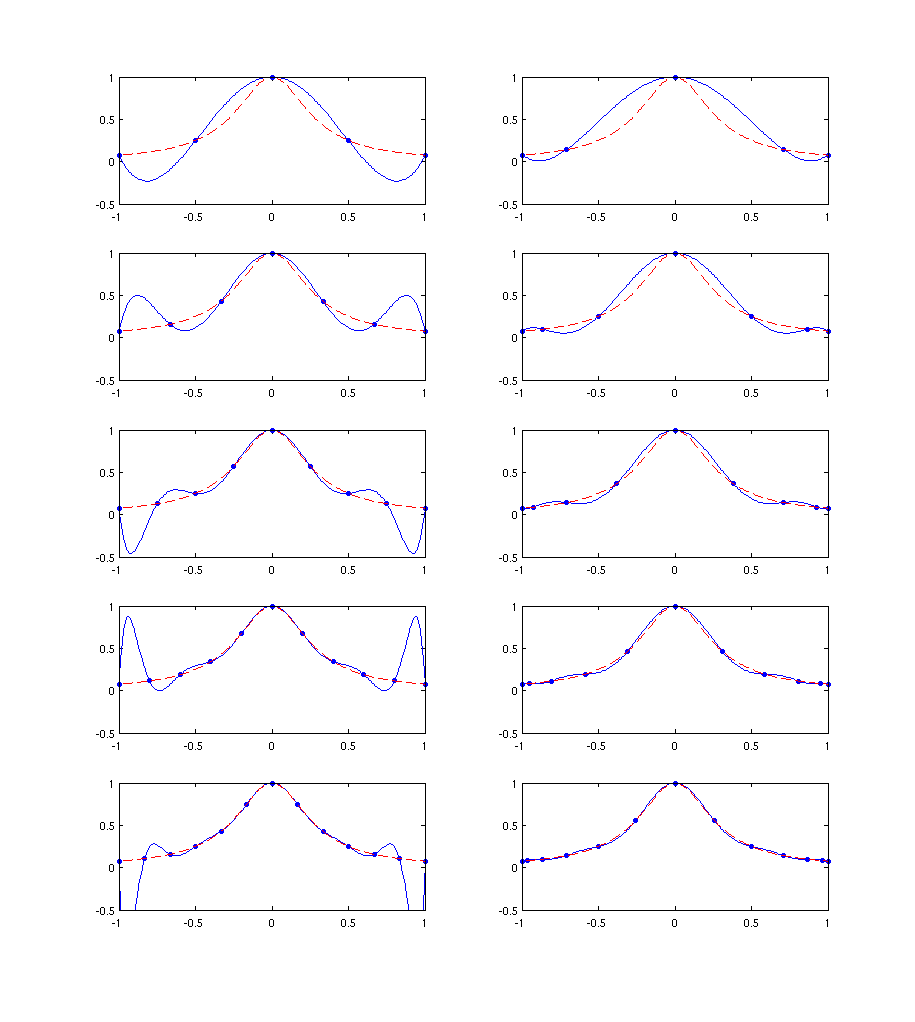
\includegraphics[scale=0.6]{num1_1_4}
		\end{figure*}
\end{aufgabe}

\end{document}
